\section{Математическое описание}

\subsection{Граф и его представление}

Граф~--- пара $G = (V, E)$, где $V$~--- конечное непустое множество вершин,
$E \subseteq V \times V$~--- множество рёбер. Граф называется ориентированным,
если каждое ребро~--- упорядоченная пара, и неориентированным в противном
случае. Ациклический граф не содержит циклов; связный ациклический
неориентированный граф является деревом, ориентированный~--- DAG
(directed acyclic graph).

Взвешенный граф задаёт функцию весов $w : E \to \mathbb{R}$, ставящую
каждому ребру вещественное число. В данной работе веса генерируются
по распределению Рэлея--Райса с параметрами, задаваемыми пользователем.

\subsection{Распределение Рэлея--Райса}

Согласно справочнику Вадзинского (п.~3.16), обобщённое распределение Рэлея
(распределение Рэлея--Райса) задаётся плотностью вероятности:
\[
    f(z) = \frac{z}{a^2}\,
           e^{-(z^2 + h^2)/(2a^2)}\,
           I_0\!\left(\frac{zh}{a^2}\right),
    \quad z \geq 0,
\]
где $a > 0$~--- параметр масштаба, $h \geq 0$~--- параметр формы,
$I_0$~--- модифицированная функция Бесселя нулевого порядка.

Для генерации случайных чисел справочник приводит следующий алгоритм, если $u_1, u_2 \sim \mathcal{N}(0,1)$~--- независимые
стандартные нормальные значения, то
\[
    z = \sqrt{(h + a u_1)^2 + (a u_2)^2}.
\]

На рис.~\ref{fig:math_distribution_compare} слева указан график из справочника, формулы которого были описаны выше, справа находится график распределения его программной реализации при $n = 1000$, равному числу вершин графа.

\begin{figure}[H]
    \centering
    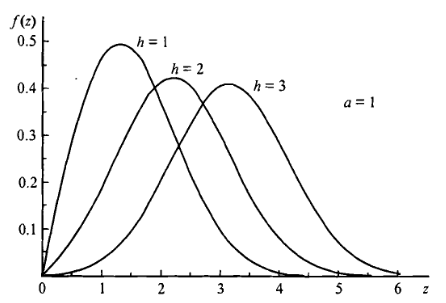
\includegraphics[width=0.48\linewidth]{images/math/dist_orig.png}%
    \hfill
    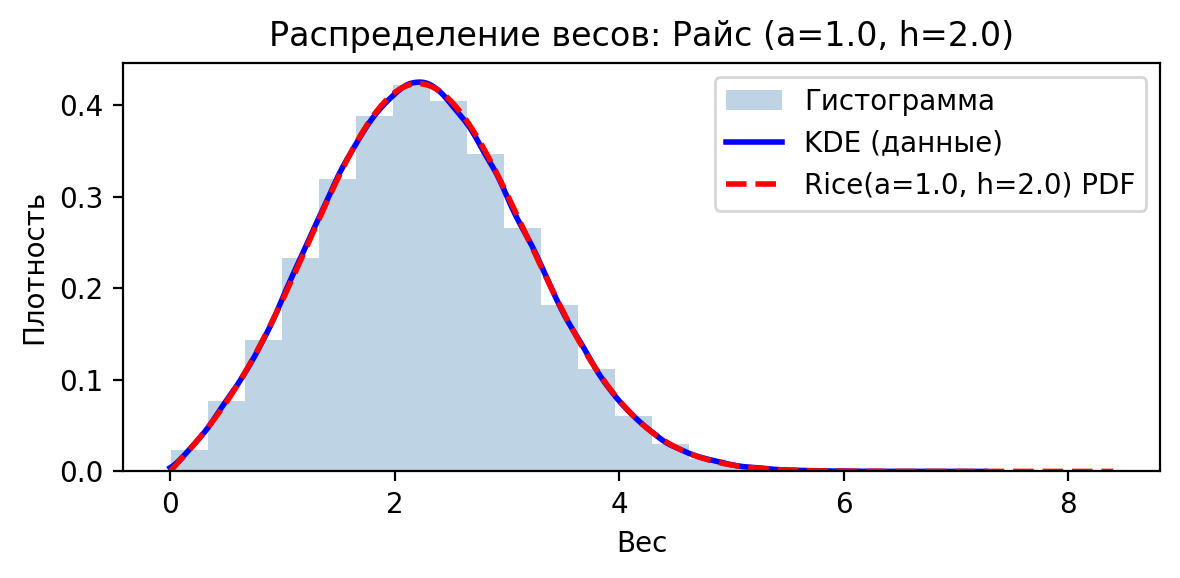
\includegraphics[width=0.48\linewidth]{images/math/dist_mine.png}
    \caption{График из справочника и распределение реализации}
    \label{fig:math_distribution_compare}
\end{figure}

Как видно из графиков, полученное распределение совпало с эталонным.

\subsection{Генерация связного ациклического графа по степеням вершин}

Пользователь задаёт число вершин~$n$ и параметры распределения $a$, $h$.
Число рёбер~$m$ не вводится напрямую.

\textbf{Шаг~1.} Для каждой вершины $i \in \{0, \ldots, n-1\}$ независимо
сэмплируется значение по формуле Вадзинского:
\[
    x_i = \sqrt{(h + a u_{i,1})^2 + (a u_{i,2})^2},
    \quad u_{i,1}, u_{i,2} \sim \mathcal{N}(0,1).
\]
Вектор $\mathbf{x} = (x_0, \ldots, x_{n-1})$ трактуется как ненормированные
веса вершин. Для перевода в вектор вероятностей применяется функция softmax
со стабилизацией :
\[
    \mathrm{softmax}(\mathbf{x})_i = p_i = \frac{e^{x_i - x_{\max}}}{\sum_{j=0}^{n-1} e^{x_j - x_{\max}}},
    \qquad \sum_{i=0}^{n-1} p_i = 1.
\]

\textbf{Шаг~2.} Итоговое число рёбер~$m$ сэмплируется из допустимого
диапазона $[n-1,\; n(n-1)/2]$, где $n-1$~--- минимум (остовное дерево),
$n(n-1)/2$~--- максимум (полный граф).

Для каждой вершины~$i$ определяется максимально допустимая степень
в топологическом порядке:
\[
    \mathit{capacity}_i = n - 1 - i.
\]
Взвешенная доля вершины~$i$: $q_i = p_i \cdot \mathit{capacity}_i$.
Вектор взвешенных долей масштабируется к сумме~$m$:
\[
    q_i \leftarrow q_i \cdot \frac{m}{\displaystyle\sum_j q_j}.
\]
Целевая степень вершины: $d_i = \lfloor q_i \rfloor$. Если после округления
$\sum_i d_i < m$, недостающие единицы последовательно прибавляются
к вершинам с наибольшей дробной частью $q_i - \lfloor q_i \rfloor$
при условии $d_i < \mathit{capacity}_i$.

\textbf{Шаг~3.} Граф строится в два прохода. В первом формируется
остовное дерево: для каждой вершины $i \geq 1$ предок выбирается
равномерно случайно из множества вершин $j < i$, для которых
остаток целевой степени $d_j > 0$; если таких вершин нет~---
равномерно из $\{0, \ldots, i-1\}$. После добавления ребра $(j, i)$
остаток целевой степени предка уменьшается: $d_j \leftarrow d_j - 1$.
Построение по индексам $j < i$ гарантирует связность и ацикличность.

Во втором проходе для каждой вершины~$i$ с $d_i > 0$ формируется
множество допустимых соседей $\{j \mid j > i,\; (i,j) \notin E\}$,
из которого случайно без возвращения выбираются
$\min(d_i,\,|\text{допустимых}|)$ вершин и добавляются соответствующие рёбра.

Веса рёбер сэмплируются по той же формуле Вадзинского.

\subsection{Эксцентриситет, центр и диаметральные вершины}

Для связного невзвешенного графа $G = (V, E)$ определим кратчайшее расстояние
$d(u, v)$ как суммарное расстояние минимального пути между~$u$ и~$v$.
Эксцентриситет вершины~--- максимальное расстояние до остальных вершин:
\[
    \varepsilon(v) = \max_{u \in V} d(v, u).
\]
На основе эксцентриситетов вводятся глобальные характеристики графа:
\[
    \mathrm{rad}(G)  = \min_{v \in V} \varepsilon(v), \qquad
    \mathrm{diam}(G) = \max_{v \in V} \varepsilon(v).
\]
Радиус графа --- множество вершин с минимальным эксцентриситетом:
\[
C(G) = \{v \mid \varepsilon(v) = \mathrm{rad}(G)\}
\]
Диаметральные вершины --- с максимальным:
\[
D(G) = \{v \mid \varepsilon(v) = \mathrm{diam}(G)\}
\]
Расстояния вычисляются алгоритмом обхода в ширину (\textit{BFS}), запускаемым из каждой вершины, алгоритмическая
сложность линейная ($O(V + E))$ для одного прохода, а итоговая сложность квадратична $O(V(V+E))$.

\subsection{Метод Шимбелла}

Пусть $A$~--- матрица весов графа размера $n \times n$: элемент $a_{ij}$
равен весу ребра $(i, j)$, если оно существует, иначе считается
неопределённым (\texttt{nullopt} в реализации). Метод Шимбелла позволяет
найти длины кратчайших и наидлиннейших путей из ровно~$k$ рёбер
для всех пар вершин одновременно.

Метод основан на переопределении двух алгебраических операций.
Операция «умножения» двух величин $a$ и $b$ заменяется их алгебраической
суммой:
\[
    a \cdot b = b \cdot a \;\Rightarrow\; a + b = b + a, \qquad
    a \cdot 0 = 0 \cdot a = 0 \;\Rightarrow\; a + 0 = 0.
\]
Операция «сложения» заменяется выбором минимального или максимального
из двух элементов:
\[
    a + b = b + a = \min(\max)\{a, b\},
\]
при этом нулевые (неопределённые) элементы игнорируются~--- минимум
или максимум выбирается из ненулевых значений.

На основе этих операций определяются два тропических матричных умножения.
Для операции $\otimes_{\min}$:
\[
    (A \otimes_{\min} B)_{ij}
    = \min_{k}\,\bigl(a_{ik} + b_{kj}\bigr),
\]
и аналогично $\otimes_{\max}$ с заменой $\min$ на $\max$. В общем виде
элемент матрицы $A^{(2)}$, полученной возведением $A$ в степень~2,
вычисляется как:
\[
    \omega_{ij}^{(2)} = \min(\max)
    \Bigl\{
        \omega_{i1}^{(1)} + \omega_{1j}^{(1)},\;
        \omega_{i2}^{(1)} + \omega_{2j}^{(1)},\;
        \ldots,\;
        \omega_{in}^{(1)} + \omega_{nj}^{(1)}
    \Bigr\}.
\]
Матрица $A^{(k)}$, вычисленная последовательным умножением начиная
с исходной матрицы $A$, содержит длины путей из ровно
$k$~рёбер для всех пар вершин. Временная сложность: $O(k \cdot n^3)$,
пространственная: $O(n^2)$.

\subsection{Подсчёт маршрутов}

Маршрут от вершины~$s$ до вершины~$t$~--- простой путь, не повторяющий
вершины. Все маршруты находятся методом обхода с возвратом (backtracking):
рекурсивный DFS с маской посещённых вершин. При достижении целевой вершины
текущий путь копируется в результат; при выходе из рекурсии вершина
снимается с отметки, что обеспечивает полный перебор всех вариантов.
Сложность в худшем случае~--- $O(n!)$, пространственная сложность $O(V)$.

\subsection{Обход рёбер в ширину}

Обход в ширину (\textit{BFS}) из вершины~$s$ посещает все вершины
графа. В основе алогитма лежит очередь~$Q$ и множество посещённых вершин~$\mathit{visited}$.
На каждом шаге вершина~$u$ извлекается из головы очереди; все
инцидентные рёбра $(u, v)$ обходятся, и каждая непосещённая вершина $v$
помечается и добавляется в хвост очереди~$Q$.

Алгоритмическая сложность линейная $O(V + E)$ и пространственная сложность $O(V)$. Результатом обхода алгоритма является
последовательность рёбер в порядке их первого посещения и вектор
расстояний $d[v]$~--- минимальное число рёбер от~$s$ до~$v$.

\subsection{Алгоритм Дейкстры}

Алгоритм Дейкстры находит кратчайшие пути от источника~$s$ до всех
вершин во взвешенном графе с неотрицательными весами рёбер.
Поддерживается вектор расстояний $d[v]$, инициализированный~$+\infty$
для всех вершин кроме~$s$: $d[s] = 0$. На каждом шаге из приоритетной
очереди (min-heap) извлекается вершина~$u$ с минимальным~$d[u]$;
для каждого ребра $(u, v)$ с весом~$w(u,v)$ выполняется релаксация:
\[
    d[v] \leftarrow \min\!\bigl(d[v],\; d[u] + w(u,v)\bigr).
\]
Если значение обновилось~--- пара $(d[v], v)$ добавляется в очередь,
а предшественник $p[v] \leftarrow u$ записывается для восстановления пути.

Кратчайший путь до целевой вершины~$t$ восстанавливается обратным
проходом по массиву~$p$: начиная с~$t$, следуем $t \to p[t] \to
p[p[t]] \to \cdots \to s$ и разворачиваем последовательность.

Алгоритмическая сложность на бинарной куче:
$O((V + E)\log{V})$, пространственная сложность $O(V)$.

\subsection{Определение сети}
Пусть $G = (V, E)$~--- орграф с одним истоком $s \in V$ и одним стоком
$t \in V$, где $s \neq t$. \textbf{Сетью} $S = (G;\, c)$ называется орграф
$G$ с заданной функцией $c : E \to \mathbb{R}_+$, сопоставляющей каждой
дуге $e \in E$ неотрицательное действительное число $c(e)$, называющееся
\textbf{пропускной способностью} этой дуги $e$.

\subsection{Поток в сети}
\textbf{Потоком} в сети $S$ называется функция $f : E \to \mathbb{R}_+$,
приписывающая каждой дуге $e \in E$ неотрицательное число $f(e)$,
для которой выполняются два условия.

Первое~--- ограничение пропускной способности: для каждой дуги $e \in E$
\[
    f(e) \leqslant c(e).
\]

Второе~--- закон сохранения потока: для каждой вершины $v \in V$,
$v \neq s, t$,
\[
    D_f(v) = \sum_{e \in A(v)} f(e) - \sum_{e \in B(v)} f(e) = 0,
\]
где $A(v)$~--- множество дуг, исходящих из $v$,
$B(v)$~--- множество дуг, входящих в $v$.

\textbf{Величиной потока} $f$ называется число
\[
    p_f = \sum_{e \in A(s)} f(e).
\]
Число $w(f) \stackrel{\mathrm{def}}{=} \mathrm{div}(f, s)$ также называется
величиной потока $f$. Дуга $(u, v)$ называется \textit{насыщенной},
если $f(u, v) = c(u, v)$.

\subsection{Алгоритм Форда--Фалкерсона}

\textbf{Теорема} (Л.\,Р.\,Форд, Д.\,Р.\,Фалкерсон, 1962).
\textit{Величина максимального потока $p_{\max}$ в сети $S$ совпадает
с минимальной пропускной способностью $r_{\min}$ её разрезов.}

Алгоритм итеративно находит увеличивающий путь от истока к стоку
в остаточной сети~--- путь, по которому остаточная пропускная
способность каждого ребра строго положительна. Величина
дополнительного потока по найденному пути:
\[
    \Delta f = \min_{(u,v) \in P} r(u,v).
\]
Для каждого ребра $(u,v)$ пути $P$ поток обновляется:
\[
    f(u,v) \leftarrow f(u,v) + \Delta f, \qquad
    f(v,u) \leftarrow f(v,u) - \Delta f.
\]
Алгоритм завершается, когда увеличивающий путь не существует.
При этом для корректной работы алгоритма требуется, чтобы пропускные способности (и стоимости) рёбер были неотрицательными.
В реализации поиск пути выполняется через BFS, что гарантирует сложность $O(V \cdot E^2)$.

\subsection{Нахождение заданного потока минимальной стоимости}
Рассмотрим задачу определения потока заданной величины $\theta$ от $s$ к
$t$ в сети $G = (S, U, \Omega, D)$, в которой каждая дуга $(x_i, x_j)$
характеризуется пропускной способностью $c(x_i, x_j) \in \Omega$ и
неотрицательной стоимостью $d(x_i, x_j) \in D$ пересылки единичного
потока из $x_i$ в $x_j$ вдоль дуги $(x_i, x_j)$.

Если $\theta > \varphi_{\max}$, где $\varphi_{\max}$~--- величина
максимального потока в сети $G$ от $s$ к $t$, то решения не существует.
При $\theta \leqslant \varphi_{\max}$ может быть определено несколько
потоков величины $\theta$. Математическая модель задачи: минимизировать
\[
    \sum_{(x_i,\, x_j) \in U} d(x_i, x_j) \cdot \varphi(x_i, x_j),
\]
где $\varphi(x_i, x_j)$~--- поток по дуге $(x_i, x_j)$, при ограничениях:

\begin{enumerate}
    \item $0 \leqslant \varphi(x_i, x_j) \leqslant c(x_i, x_j)$
          для всех $(x_i, x_j) \in U$;
    \item для начальной вершины $s \in S$ (уравнение истока):
          \[
              \sum_{x_j \in S} \varphi(s, x_j) -
              \sum_{x_j \in S} \varphi(x_j, s) = \theta
          \]
    \item для конечной вершины $t \in S$ (уравнение стока):
          \[
              \sum_{x_j \in S} \varphi(t, x_j) -
              \sum_{x_j \in S} \varphi(x_j, t) = -\theta
          \]
    \item для любой другой вершины $x_j \neq s, t$ (условие сохранения потока):
          \[
              \sum_{x_i \in S} \varphi(x_j, x_i) -
              \sum_{x_i \in S} \varphi(x_i, x_j) = 0
          \]
\end{enumerate}

\subsection{Теорема Кирхгофа}

Пусть $G = (V, E)$~--- связный неориентированный граф без петель и кратных
рёбер, $|V| = n$. \textit{Матрица Кирхгофа} $B = B(G) = (b_{ij})_{n \times n}$ определяется как:
\[
    B = D - A(G),
\]
где $D = \mathrm{diag}(\deg v_1, \ldots, \deg v_n)$~--- диагональная матрица
степеней вершин, $A(G)$~--- матрица смежности графа $G$. Явно:
\[
    b_{ij} =
    \begin{cases}
        \deg v_i, & i = j, \\
        -1,       & i \neq j,\ v_i \sim v_j, \\
        0,        & i \neq j,\ v_i \not\sim v_j.
    \end{cases}
\]

Сумма элементов каждой строки (и каждого столбца) матрицы $B$ равна нулю,
поэтому $\det B = 0$ и $\lambda_i = 0$~--- собственное значение $B$. Для связного графа
кратность нулевого собственного значения равна единице, остальные
$n - 1$ собственных значений строго положительны.

\textbf{Лемма} \textit{Все алгебраические дополнения
элементов матрицы Кирхгофа равны между собой.}

\textbf{Теорема} (матричная теорема Кирхгофа). \textit{Число различных
остовных деревьев связного графа $G$ равно любому определютелю его матрицы
Кирхгофа:}
\[
    \tau(G) = \det B_{ii},
\]
\textit{где $B_{ii}$~--- матрица $B$ с удалённой $i$-й строкой и $i$-м
столбцом.}

Алгоритмическая сложность: $O(n^3)$, пространственная: $O(n^2)$.

\subsection{Алгоритм Борувки}

Алгоритм Борувки~--- алгоритм построения минимального остовного дерева
во взвешенном связном неориентированном графе $G = (V, E)$ с функцией
весов $w : E \to \mathbb{R}$. Впервые опубликован О.\,Борувкой в 1926 году.

\textit{Минимальное остовное дерево} (МОД)~--- остовное дерево
$T \subseteq E$ с минимальным суммарным весом $\sum_{e \in T} w(e)$.

\textbf{Описание алгоритма.}
\begin{enumerate}
    \item Изначально каждая вершина графа~--- тривиальное дерево
          (компонента из одной вершины); множество рёбер остова $T = \varnothing$.
    \item Для каждой компоненты $C_k$ находится минимальное по весу ребро,
          инцидентное ей и соединяющее её с другой компонентой.
          При равенстве весов среди кандидатов выбирается ребро
          с наименьшим индексом, что исключает добавление цикла.
          Все найденные рёбра добавляются в $T$;
          компоненты, соединённые этими рёбрами, объединяются.
    \item Шаг~2 повторяется, пока в графе не останется одна компонента.
\end{enumerate}

\textbf{Теорема.} \textit{Алгоритм Борувки строит минимальное остовное дерево.}

Алгоритмическая сложность: $O(E \log V)$, пространственная: $O(V + E)$.

\subsection{Код Прюфера}

\textbf{Кодирование.} Пусть $T = (V, E_T)$~--- дерево с вершинами
$V = \{1, \ldots, n\}$. Код Прюфера~--- последовательность
$A = (A[1], \ldots, A[n-2])$, строящаяся следующим образом:
на каждом из $n - 2$ шагов выбирается висячая вершина $v$ с минимальным
номером ($\deg v = 1$), в код записывается её единственный сосед
$\Gamma(v)$, после чего вершина $v$ удаляется из дерева:
\[
    A[i] = \Gamma\!\left(\min\{k \in V \mid \deg(k) = 1\}\right),
    \quad V \leftarrow V \setminus \{v\}, \quad i = 1, \ldots, n-2.
\]
В конце остаются ровно две вершины; информация о последнем ребре
не хранится, поскольку восстанавливается однозначно.

Код Прюфера~--- наиболее экономное по памяти представление помеченного
дерева: последовательность из $n - 2$ чисел кодирует $n^{n-2}$ различных
помеченных деревьев (формула Кэли).

\textbf{Декодирование.} По коду $A = (A[1], \ldots, A[n-2])$
восстанавливается дерево $T = (V, E_T)$. Поддерживается множество
«свободных» вершин $B = \{1, \ldots, n\}$.
На каждом шаге~$i$ выбирается наименьшая вершина $v \in B$, не
встречающаяся в остатке кода $A[i..n-2]$; добавляется ребро $(v, A[i])$,
вершина $v$ удаляется из $B$:
\[
    v = \min\{k \in B \mid \forall\, j \geq i : k \neq A[j]\},
    \quad E_T \leftarrow E_T \cup \{(v, A[i])\},
    \quad B \leftarrow B \setminus \{v\}.
\]
После $n - 2$ шагов в $B$ остаются ровно две вершины~--- они соединяются
последним ребром. Алгоритмическая сложность кодирования и декодирования:
$O(n \log n)$, пространственная: $O(n)$.

Веса рёбер МОД сохраняются при кодировании: каждому ребру
$(u, v) \in E_T$ сопоставляется вес $w(u, v)$; при декодировании
веса восстанавливаются по соответствию между рёбрами исходного
остова и рёбрами, добавляемыми на каждом шаге декодирования.

\subsection{Минимальная раскраска графа}

\textit{Правильная раскраска} графа $G = (V, E)$~--- отображение
$c : V \to \{1, \ldots, k\}$ такое, что для любого ребра $(u, v) \in E$
выполняется $c(u) \neq c(v)$. Минимальное число цветов, при котором
существует правильная раскраска, называется \textit{хроматическим числом}
$\chi(G)$.

Нахождение $\chi(G)$ является NP-трудной задачей в общем случае.
В данной работе реализован точный алгоритм на основе полного перебора
с отсечениями (backtracking): вершины обходятся в фиксированном порядке;
каждой вершине последовательно назначается наименьший допустимый цвет~---
такой, которым не окрашен ни один из уже обработанных соседей.
Если при некотором числе цветов~$k$ раскраска найдена, алгоритм
повторяется для $k - 1$ цветов; процедура продолжается до тех пор,
пока раскраска при $k - 1$ цветах не окажется невозможной.

Алгоритмическая сложность в худшем случае: $O(k^V)$,
пространственная: $O(V)$.


\subsection{Эйлеров граф}

Граф $G = (V, E)$ называется \textit{эйлеровым}, если в нём существует
замкнутый маршрут, проходящий по каждому ребру ровно один раз~---
\textit{эйлеров цикл}. Граф называется \textit{полуэйлеровым}, если
такой маршрут существует, но не является замкнутым~--- \textit{эйлеров путь}.

\textbf{Теорема} (Эйлер, 1736). \textit{Связный неориентированный граф
является эйлеровым тогда и только тогда, когда степень каждой вершины чётна:}
\[
    \forall v \in V : \deg(v) \equiv 0 \pmod{2}.
\]
\textit{Граф является полуэйлеровым тогда и только тогда, когда он
связен и имеет ровно две вершины нечётной степени; эти вершины служат
началом и концом эйлерова пути.}

Множество вершин нечётной степени обозначим:
\[
    \mathrm{Odd}(G) = \{v \in V \mid \deg(v) \equiv 1 \pmod{2}\}.
\]
Тогда: $G$ эйлеров $\Leftrightarrow$ $\mathrm{Odd}(G) = \varnothing$;
$G$ полуэйлеров $\Leftrightarrow$ $|\mathrm{Odd}(G)| = 2$.

\subsection{Достройка графа до эйлерова}

Если $\mathrm{Odd}(G) \neq \varnothing$, граф модифицируется
добавлением рёбер. Процедура состоит из двух этапов.

\textbf{Этап~1.} Если граф несвязен, ненулевые компоненты связности
$C_1, C_2, \ldots, C_p$ соединяются цепочкой дополнительных рёбер:
для каждого $k = 2, \ldots, p$ добавляется ребро
$(u_{k-1},\, u_k)$, где $u_k \in C_k$~--- произвольный
представитель компоненты. После этого граф становится связным.

\textbf{Этап~2.} Пока $|\mathrm{Odd}(G)| > 2$, вершины из
$\mathrm{Odd}(G)$ разбиваются на пары и между каждой парой
добавляется ребро. Каждое добавление уменьшает
$|\mathrm{Odd}(G)|$ ровно на два: оба конца нового ребра меняют
чётность степени. Если $|\mathrm{Odd}(G)| = 2$, добавляется
одно замыкающее ребро ,причем если такое ребро уже существует в графе, то для замыкания полуэйлерова графа до эйлерова оно не дублируется, а извлекается (удаляется) из системы~--- граф становится эйлеровым.

\subsection{Алгоритм Иерхольцера}

Алгоритм Иерхольцера находит эйлеров цикл (или путь) в графе,
удовлетворяющем условию теоремы Эйлера. Используется итеративная
реализация на основе стека.

Для старта выбирается вершина $s \in \mathrm{Odd}(G)$ при
полуэйлеровом графе, иначе~--- произвольная вершина с ненулевой
степенью. Поддерживается стек $\mathit{stk}$, вектор использованных
рёбер $\mathit{used} : E \to \{0,1\}$ и указатели
$\mathit{ptr}[u]$~--- индекс следующего непросмотренного ребра
вершины $u$.

На каждом шаге рассматривается вершина $u = \mathit{stk.top}()$.
Если существует неиспользованное ребро $(u, v)$~--- оно помечается
($\mathit{used}[\mathrm{id}] \leftarrow 1$) и $v$ помещается на стек.
Если таких рёбер нет~--- $u$ снимается со стека и дописывается
в маршрут $\pi$. По завершении $\pi$ разворачивается.

Корректность проверяется двумя условиями:
\[
    |\pi| = |E| + 1
\]
Алгоритмическая сложность: $O(V + E)$, пространственная: $O(V + E)$.

\subsection{Фундаментальная система разрезов}

Пусть $T = (V, E_T)$~--- остовное дерево графа $G = (V, E)$.
Удаление ребра $e \in E_T$ разбивает $T$ на два поддерева с
множествами вершин $A$ и $B = V \setminus A$.
\textit{Фундаментальный разрез} ребра $e$~---
множество рёбер исходного графа, пересекающих это разбиение:
\[
    S(e) = \bigl\{(u, v) \in E \;\big|\;
    (u \in A \wedge v \in B) \vee (u \in B \wedge v \in A)\bigr\}.
\]
Заметим, что $e \in S(e)$ всегда, поскольку ребро остова
само пересекает разбиение.

Совокупность фундаментальных разрезов по всем рёбрам остова
образует \textit{фундаментальную систему разрезов} (ФСР):
\[
    \mathcal{F}(T) = \bigl\{S(e) \mid e \in E_T\bigr\}.
\]
$|\mathcal{F}(T)| = |E_T| = |V| - 1$.
Разрезы из $\mathcal{F}(T)$ линейно независимы
и порождают пространство разрезов графа размерности $|V|-1$.

\subsection{Симметрическая разность разрезов}

Произвольный разрез графа выражается через фундаментальные
с помощью операции \textit{симметрической разности}:
\[
    S_1 \triangle S_2 = (S_1 \setminus S_2) \cup (S_2 \setminus S_1)
                      = (S_1 \cup S_2) \setminus (S_1 \cap S_2).
\]
Операция $\triangle$ ассоциативна и коммутативна. Ребро $(u,v)$ входит в симметрическую разность
подмножества разрезов тогда и только тогда, когда оно встречается
в нечётном числе слагаемых:
\[
    S(e_{i_1}) \triangle \cdots \triangle S(e_{i_k})
    = \Bigl\{(u,v) \in E \;\Big|\;
      \sum_{j=1}^{k} \mathbf{1}\bigl[(u,v) \in S(e_{i_j})\bigr]
      \equiv 1 \pmod{2}\Bigr\}.
\]
